The goal was to achieve a muscle activation driven pointing task using a 2-DoF, 6-muscle arm model. 
In addition to muscle-induced torques, pure joint torques could compensate for the model weaknesses.

The first term of the objective function (Eq.~\ref{eq:cost_ex1}) corresponds to the pointing tasks described by a Mayer term (\comment{heaviest weight}{Est-ce que ce n'est pas étrange d'avoir un poids sur les deux? pourquoi pas 1e5 et 1?}), to superimpose two markers, the first one fixed in the ulna system of coordinates and the second one fixed in the scene.
The second and third were added for control regularization (muscle activation and torques) and the fourth one for state regularization:

%
%\begin{table}[h!]
%\caption{\small Objective terms of the activation-driven pointing task. The names of the functions correspond to the nomenclature used in \textit{Bioptim}.}
%\label{tab:Muscle_activation_driven_pointing_task}
%\centering
%\begin{tabular}{c c c c}
%\toprule 
%& Type & Function & Weight \\ 
%\midrule
%$\#1$ & Mayer & ALIGN\_ MARKERS & $1e6$ \\ 
%\midrule
%$\#2$ & Lagrange & MINIMIZE\_ MUSCLE\_ CONTROL & $1e1$ \\ 
%\midrule
%$\#3$ & Lagrange & MINIMIZE\_ TORQUE & $1e1$ \\ 
%\midrule
%$\#4$ & Lagrange & MINIMIZE\_ STATE & $1e1$ \\
%\bottomrule
%\end{tabular}
%\end{table}
%
\[
\resizebox{0.9\columnwidth}{!}{$
\begin{aligned}
	\mathcal{C} = &1e6~\text{\comment{align}{Selon Jenn, track serait un meilleur choix de mot}\_markers}\\
	&+ \int 10~(\text{min\_muscle\_ctrl}+\text{min\_torque}+\text{min\_state}),
\end{aligned}
$}
\addtag
\label{eq:cost_ex1}
\]
%
\noindent where the names of the objective terms correspond to the nomenclature used in \textit{Bioptim}.
The movement lasted for 2~seconds and was discretized using \comment{51}{Donc 52 nodes? ça me semble étrange} shooting nodes.
The problem was solved using IPOPT and ACADOS resulting in two significantly different solutions.
ACADOS provided a 16 times smaller optimized cost (Tab.~\ref{tab:Perfs_and_detailed_implementations_of_each_example}), which illustrate the pitfalls of local minima as well as the benefits of having straightforward access to different solvers.  
Indeed, the ACADOS-based solution (Fig.~\ref{fig:snapshots_activation_driven_pointing}, top) makes good use of gravity to minimize the control inputs, while the IPOPT-based solution (Fig.~\ref{fig:snapshots_activation_driven_pointing}, bottom) moved the arm in the opposite direction and was stuck in a local minimum (still achieving the task though). 
It is worth mentioning that for the purpose of this illustration, no constraint was given about the shoulder range of motion to ensure physiological muscle trajectories. 

 
 

%
\begin{figure*}[t!]
\centering
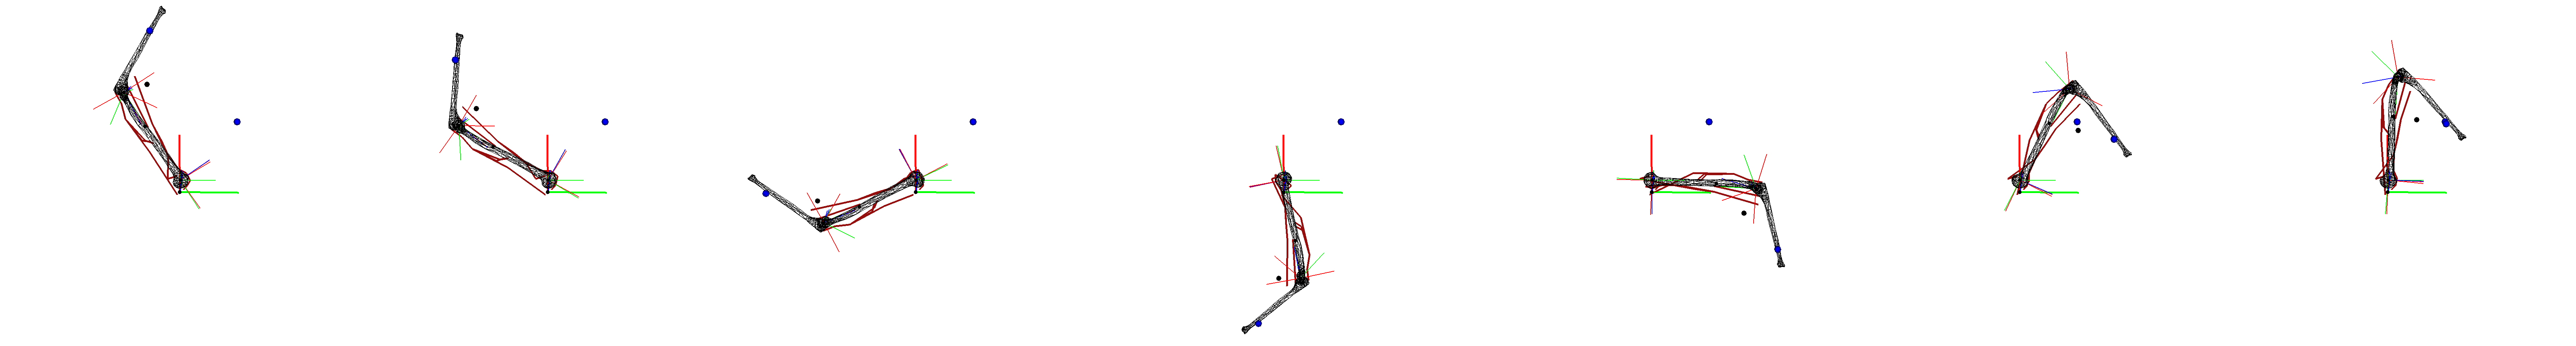
\includegraphics[width=\textwidth]{figures/activation_pointing_snapshots_acados.png}\\
\vspace*{0.5em}
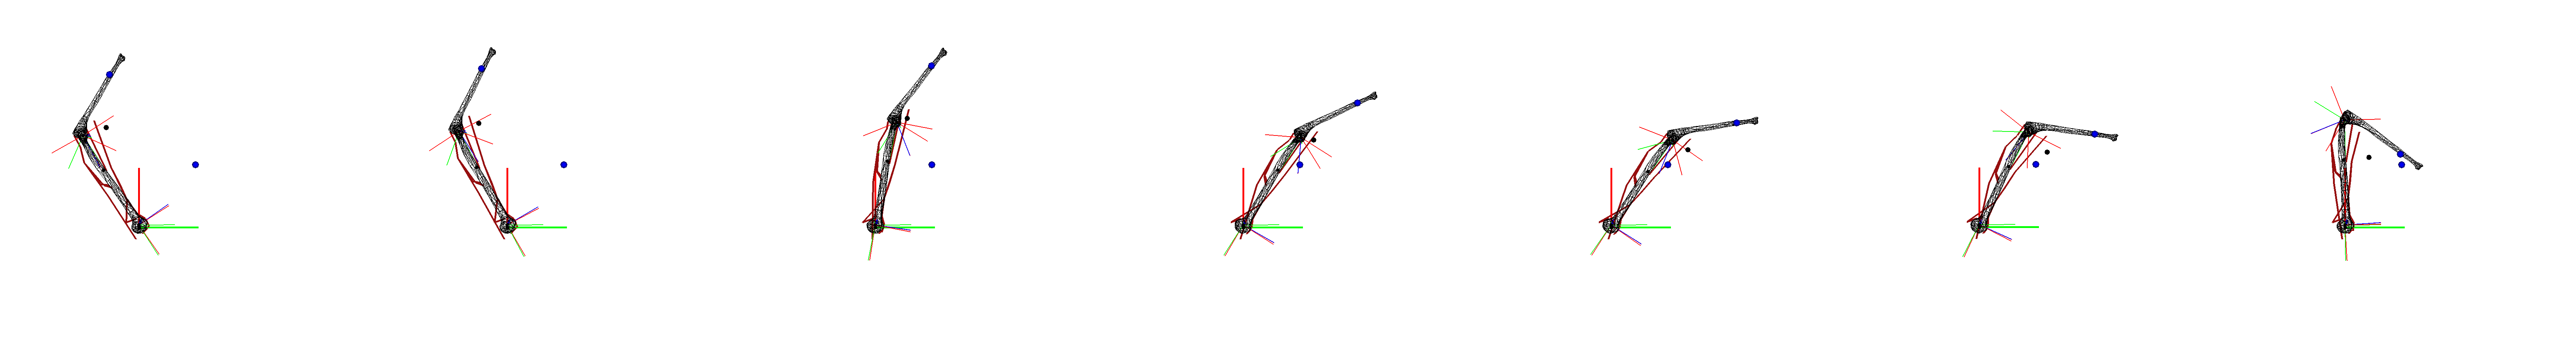
\includegraphics[width=\textwidth]{figures/activation_pointing_snapshots_ipopt.png}
\caption{Snapshots of an optimized muscle activation driven pointing task. Top: using ACADOS. Bottom: using IPOPT.}
\label{fig:snapshots_activation_driven_pointing}
\end{figure*}
%









